
\section{IPOL web interface}

current version is 3.0.

\subsection{Introduction}
The IPOL demo Web interface has been developed with HTML5, CSS3 \miguel{Add a comma before 'and' in enumerations} and Jquery. 
This web page is responsible for letting the users execute demos using either blobs 
from the demo or blobs uploaded by the user. \miguel{Rewrite: It allows the users to execute the IPOL algorithm's with an ergonomic interface. The users can use their own data or the examples offered by each of the demos.}

\miguel{We shall describe the modules of which the web interface is made, its flow diagram, how the asynchronous calls work, and the data types accepted.}


\section{Modules}
This section will try to explain the different modules existing in the demo app. All of these
 modules are divided across the javascript files of the application.
\miguel{Rewrite: The Javascript application is made of several modules:}
\begin{itemize}
	\item Inputs.
	\item Upload.
	\item Editor.
	\item Parameters.
	\item Run.
	\item Results.
	\item Helpers. \miguel{Remove the final dot at the end of each item}
\end{itemize}

Each of them is described in the following sections.

\subsection{Inputs}
This module will do everything \miguel{'Everything' is too vague.} related to the demo blobs. As it is the starting point of the 
application \miguel{I don't get what you mean with the 'starting point of the application'. }it will also make the Async calls needed to obtaing data from the demo using id \miguel{its ID} from the URL, like \miguel{the same way as } demoinfo 
and blobs back-end modules. These two calls will obtaing the information necesary \miguel{necessary. Use a spellchecker.} to execute the demo, letting \miguel{allowing} the 
user choose along the way \miguel{along the way? what's that?} the input blobs, edit these blobs \miguel{and comma} and tweak demo execution parameters.
This input module will let \miguel{Do not write in future tense. Change it to 'allows the user...'. You describe what already exist now, not in the future.} the user choose among blobs that the demo provides. These blobs will be either images, video \miguel{videos} \miguel{add commma} or 
audio blobs primarily. It will \miguel{Write in present tense. Describe only what has been done, not in the future} display a line of blobs or sets of blobs to choose from.


\subsection{Upload}
If the user wants to use their \miguel{If the users want to use their} own blobs for the demo this module will let you \miguel{Not future. Do not use 'you'. Write more formal} upload them. Every demo has predefined 
upload slots each with their own characteristics \miguel{Add some examples of these characteristics}. The user will \miguel{Not future} be able to upload a \miguel{the} minimum required number of uploads.
This module will \miguel{not future} listen for events en \miguel{in} every upload slot and get the file information in order to upload them when the run 
button is pressed.

\subsection{Editor}
This module will \miguel{Change ALL future tenses and describe only what is done} load after the user selects a set of blobs to run the demo with or when the users upload their blobs. It will load a view of the chosen blobs where there will be a zoom and crop functions when the sets have 
one blob per set. When the sets have more than one blob per set, the user will also be able a \miguel{will have the possibility to compare them with the corresponding 'Compare button', but not to crop an area.} compare button but not a crop 
option.

\subsection{Parameters}
This module will print itself after \miguel{renders the parameters of the demo described in the DDL after} the user chooses the blobs to use with the demo. It will print itself after the editor \miguel{The 'editor' hasn't been yet define} and will 
contain as many parameters as the DDL specifies. Parameters have their own specification as well as different types.

\subsection{Run}
This module will compile \miguel{Do not use 'compile', because this is used to compile the code} all the blobs and requirements needed to run the demo and will send this information to the demorunner \miguel{DemoRunner} module. Then it will wait \miguel{block} until there is a response and print the results \miguel{Do not use 'print'. Be more specific.}.

\subsection{Results}
This module will print the results the demorunner gives back \miguel{returns} letting the user compare the input and results.

\subsection{Helpers}
This module act as an interface for common utility methods like read and write to sessionStorage, make http \miguel{HTTP} requests and 
read the origin \miguel{You don't say which is an origin and what origins are possible} of the chosen blobs for the demo.

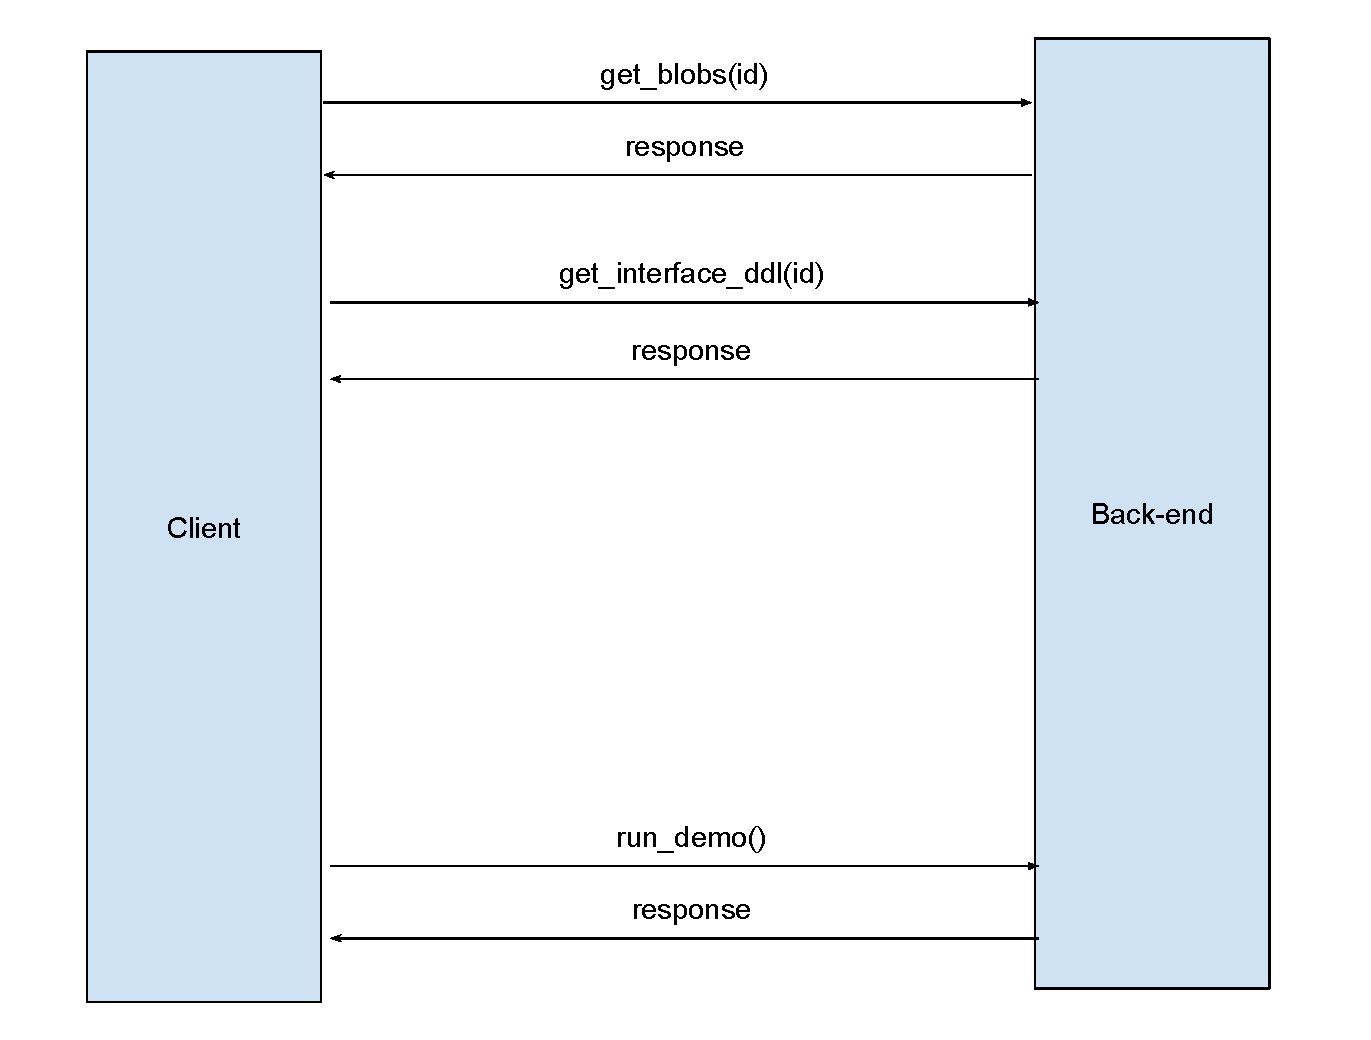
\includegraphics[width=\textwidth]{images/client_server_interaction}
\miguel{Convert the graphics into a figure with a caption. Also, refer to it in the text using {\tt ref}}

%--------------------------------------------------------------------------------

\section{Flow diagram}
The first thing the application will do when loaded is look for an id which \miguel{When the application is loaded, the XXX module will locate the demo according to its ID} represents
the demo id to be represented \miguel{Reread and rewrite}. This ID is a get parameter of the URL.
At the same time \miguel{As the same time it reads the ID?} the main file, demo.js will load the different html files into the DOM. They have been divided into various \miguel{several} files to improve mantainability and coupling.

After all this \miguel{Do not write 'all this'} is loaded, the app will continue adding the main section to the DOM,
 containg in this case the blobs viewer and the blobs upload dialog. At the same time \miguel{At the same time? Events? Be more specific}, the 
 the information regarding the current demo, responses from \miguel{the} blobs \miguel{Blobs}  and demoInfo modules 
 will be saved at \miguel{in} sessionStorage.
 
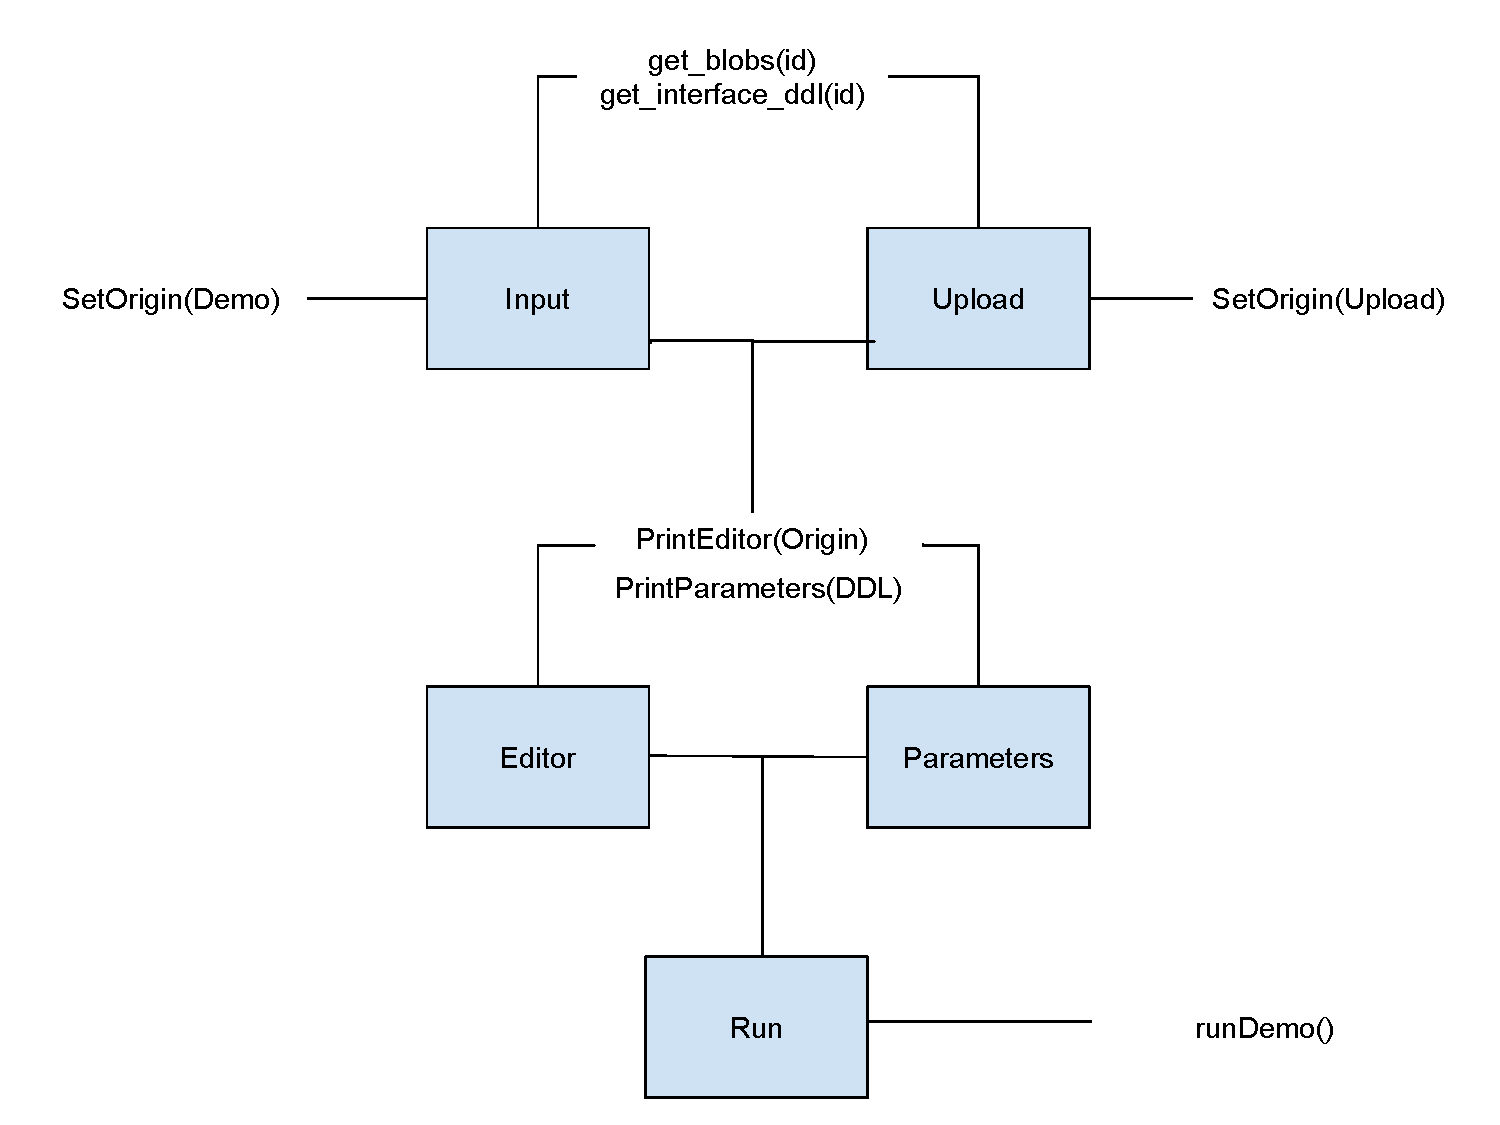
\includegraphics[width=\textwidth]{images/flow}

As the diagram shows \miguel{Put a footer}, either input or upload modules will pass information to the following modules. Each will set a variable in sessionStorage 
that will indicate if the user has chosen to upload blobs for the demo or a default blob from the list. 

After the user chooses a blob, the editor and parameter modules will load independently and wait for changes. Editor \miguel{The Editor control} will allow to either 
zoom, crop \miguel{add comma}  and compare blobs when \miguel{remove well, add 'if'} possible, as well as do inpainting operations when the demo requires it. The parameters will allow  
tweaking \miguel{The configure the parameter controls, but that's not tweaking} according to ddl \miguel{to the DDL} specification. Parameter values will be stored in a variable for refreshing feature purpose as the ddl states. \miguel{This last sentence is hard to understand.}

After the user hits the run button an http post will be executed to run the demo and send the necessary information and wait for a response. 
When the response is obtained it will either print the results interface or the error message.

%--------------------------------------------------------------------------------

\subsection{External modules}

The IPOL demo Web interface uses external libraries for extra functionalities.
Currently it uses:

\begin{itemize}
\item Cropper.js: Cropper.js it is a simple image cropping JQuery plugin. It is used in the editor panel with the image blobs.
\end{itemize}

%--------------------------------------------------------------------------------

\subsection{Async calls}
The IPOL demo Web interface uses Async calls to get the necessary information from the IPOL server and use it \miguel{'and use it' is redundant}.

The current version uses Async calls for:
\begin{itemize}
\item Get the demo ddl: Used to show the inputs description and the upload modal in the Inputs panel, also uses this information to show the parameters.
\item Get blobs: Used to show the blobs in the inputs panel.
\item Run demo: It will send all parameters needed to run the demo and will responde with either the results of the demo or an error response.
\end{itemize}

%--------------------------------------------------------------------------------

\subsection{Data types}
The IPOL platform supports mainly images, but recent updates include audio and video files to use in demos \miguel{You're describing the new interface. Thus, it doesn't make sense to say that it supports mainly images}. The new web interface 
allows to choose a set with any combination of images, audio and video. Depending on the data types and sets length options will vary. 
If a set contains multiple images, the user will be able to compare and make zoom using any image on the set. If the user chooses a set with only 
one image blob, options will depend on DDL limitations and will include zoom and crop features, as well as inprinting editing.

In case of uploading an audio or video file, it wont have a visual representation at the moment \miguel{But they will. It's a work in progress. Do not document that we don't support it.}, only videos and audio files in the default set from the demo will have a visual representation.

\miguel{In general, please improve the writing and be more specific.}
